\documentclass{article}
\usepackage[utf8]{inputenc}
\usepackage[spanish]{babel}
\usepackage{listings}
\usepackage{graphicx}
\graphicspath{ {images/} }
\usepackage{cite}

\begin{document}

\begin{titlepage}
    \begin{center}
        \vspace*{1cm}
            
        \Huge
        \textbf{Manual de usuario - Informatica II.}
            
        \vspace{0.5cm}
        \LARGE
            
        \vspace{1.5cm}
            
        \textbf{Luis Miguel Gil Rodriguez.}
        \\
        \textbf{Maverick Sossa Tobon.}
        \vfill
        \vspace{0.8cm}
            
        \Large
        Despartamento de Ingeniería Electrónica y Telecomunicaciones\\
        Universidad de Antioquia\\
        Medellín\\
        Septiembre de 2021
            
    \end{center}
\end{titlepage}
\tableofcontents
\newpage
\section{Manual de usuario.} \label{intro}
En este corto pero eficiente manual de usuario podrás aprender cómo utilizar nuestro software para mostrar una bandera en una matriz de 16X16 LEDs, como lo mostraremos en los siguientes ejemplos:
\begin{figure}[h]
  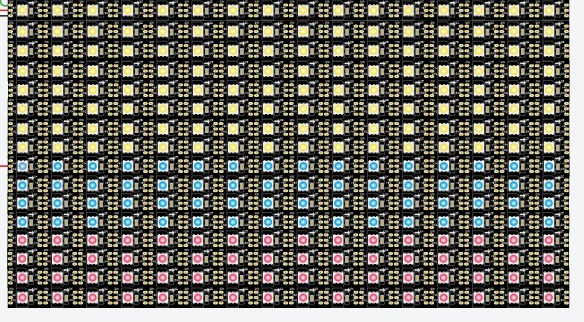
\includegraphics[width=10cm]{Colombia.jpg}
  \centering
  \caption{La bandera de Colombia en la matriz de LEDs.}
  \label{fig:Colombia}
\end{figure}
\begin{figure}[h]
  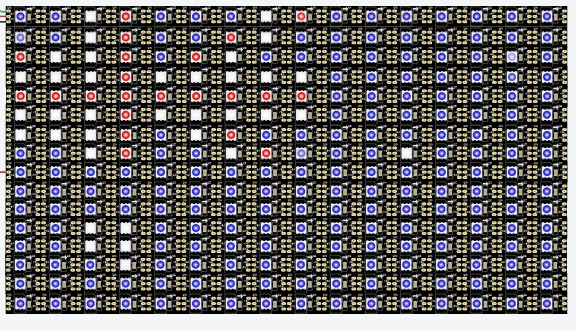
\includegraphics[width=10cm]{Australia.jpg}
  \centering
  \caption{La bandera de Australia en la matriz de LEDs.}
  \label{fig:Colombia}
\end{figure}
Luego de haber ejecutado satisfactoriamente el programa de redimensionamiento de Imágenes, iremos a la Carpeta DB, ubicada dentro del proyecto de Qt, en la cual podemos encontrar archivo de texto titulado “ImgResize.txt”, allí podremos encontrar la información de la imagen redimensionada dividida en 3 matrices unidimensionales, las cuales representara la intensidad del Rojo, Verde o Azul en números enteros de 0 a 255
\\
Después de esto, procedemos a abrir el proyecto de Tinkercad, presionaremos el Botón “Código”, ubicado en la parte superior derecha de la pagina y pegaremos la información del archivo “ImgResize.txt” en la línea numero 19, de lo contrario el programa no funcionara de forma correcta.
\\
\\
Luego de esto, podemos presionar en el botón “Iniciar simulación”, el cual se encuentra al lado derecho del botón “Código”.
Si desea evidenciar el valor que se le esta asignando a cada Píxel, puede dar un click en el Monitor Serial de Tinkercad, el cual se encuentra en la parte inferior del Código.
Debe esperar hasta que el software envíe la información a cada LED de la matriz, una vez este proceso termine, inmediatamente se vera reflejado el resultado en la matriz. 

\bibliographystyle{IEEEtran}
\bibliography{references}
\end{document}
